\chapter{Les interactions entre espèces}\label{ch:b1:species-interactions}

En 1963, sur une côte rocheuse du Pacifique, un jeune écologue se mit à
rejeter à la mer chaque étoile de mer qu'il trouvait sur une portion de
rocher, et continua ainsi pendant des années. L'étoile de mer mangeait
les moules. Sans elle, les moules s'étendirent vers le bas sur le
rocher et évincèrent les balanes, les patelles, les chitons et les
algues qui y vivaient~; une \omterm{def:b1:ecosystem-organization:ecosystem}{biocénose} de quinze espèces tomba à huit. Un
seul prédateur, ni abondant ni grand, maintenait tout l'assemblage en
place. Les espèces ne se partagent pas seulement un lieu~; elles s'en
disputent, se mangent, vivent l'une dans l'autre et l'une sur l'autre,
et dépendent l'une de l'autre, et la \omterm{def:b1:ecosystem-organization:ecosystem}{biocénose} est la somme de ces
interactions. Ce chapitre les classe, donne les modèles quantitatifs de
la \omterm{def:b1:species-interactions:types}{compétition} et de la \omterm{def:b1:species-interactions:types}{prédation} qu'une première année peut traiter,
et montre par des expériences comment une seule interaction peut
façonner tout un \omterm{def:b1:ecosystem-organization:ecosystem}{écosystème}.

\section{Une classification des interactions}

\begin{definition}[Les interactions interspécifiques]\label{def:b1:species-interactions:types}
\index{competition@compétition}\index{predation@prédation}\index{parasitisme}\index{mutualisme}\index{commensalisme}
Une interaction entre deux espèces se classe par son effet sur
chacune~: $+$ (bénéfice), $-$ (préjudice) ou $0$. La
\emph{compétition} ($-/-$)~: les deux emploient une ressource rare. La
\emph{prédation} ($+/-$)~: l'une tue et mange l'autre~; l'\emph{herbivorie}
($+/-$) quand le mangé est une plante et survit d'ordinaire~; le
\emph{parasitisme} ($+/-$) quand l'exploiteur vit sur ou dans un hôte
qu'il ne tue pas aussitôt. Le \emph{mutualisme}
($+/+$)~: les deux y gagnent. Le \emph{commensalisme} ($+/0$)~: l'une y
gagne, l'autre n'est pas affectée. L'\emph{amensalisme} ($-/0$)~: l'une
subit un préjudice, l'autre n'est pas affectée. Toute interaction est
une pression de sélection sur les deux partenaires, et leur adaptation
réciproque au fil des générations est la \emph{coévolution}.
\end{definition}

\begin{example}[Un seul arbre, les six interactions]\label{ex:b1:species-interactions:oak}
Un chêne fait concurrence à ses voisins pour la lumière~; ses glands
sont mangés par les geais (\omterm{def:b1:species-interactions:types}{prédation}) et ses \omterm{def:b1:flowering-plant-organization:organs}{feuilles} par les chenilles
(herbivorie)~; le gui puise sa sève (\omterm{def:b1:species-interactions:types}{parasitisme})~; ses \omterm{def:b1:flowering-plant-organization:organs}{racines} échangent
des sucres contre du phosphate avec un champignon (\omterm{def:b1:species-interactions:types}{mutualisme})~; des
fougères poussent sur son écorce, qui ne leur sert que de perchoir
(\omterm{def:b1:species-interactions:types}{commensalisme})~; et son ombre tue l'herbe qui est dessous
(amensalisme).
\end{example}

\section{La compétition}

\begin{definition}[La compétition interspécifique]\label{def:b1:species-interactions:competition}
\index{exclusion competitive@exclusion compétitive}\index{partage des niches}\index{deplacement de caractere@déplacement de caractère}
Deux espèces sont en \omterm{def:b1:species-interactions:types}{compétition} quand toutes deux emploient une
ressource --- nourriture, lumière, eau, espace, sites de nidification
--- dont l'offre limite leur croissance. La \omterm{def:b1:species-interactions:types}{compétition} peut se faire
par \emph{exploitation} (chacune prend ce que l'autre aurait employé)
ou par \emph{interférence} (agression directe, toxines, territoires).
Son issue suit le \emph{principe d'exclusion compétitive}~: deux
espèces qui ont besoin de la même ressource limitante et de la même
façon ne peuvent coexister indéfiniment dans un milieu stable~; la
meilleure compétitrice élimine l'autre. Les compétitrices qui
coexistent diffèrent donc par la \omterm{def:b1:ecosystem-organization:niche}{niche} (\emph{partage des \omterm{def:b1:ecosystem-organization:niche}{niches}}) --- et
là où deux espèces se recouvrent, elles divergent souvent davantage par
la forme que là où chacune vit seule (\emph{déplacement de caractère}).
\end{definition}

\begin{proposition}[Le modèle de compétition de Lotka--Volterra]\label{prop:b1:species-interactions:lotka}
Faisons croître deux espèces de façon logistique
(\cref{ch:b1:populations}) et comptons chaque individu de l'espèce 2
pour $\alpha$ individus de l'espèce 1 dans l'usage de la ressource de
l'espèce 1, et chaque individu de l'espèce 1 pour $\beta$ de l'espèce 2~:
\[
\frac{\dd N_1}{\dd t} = r_1 N_1\left(1 - \frac{N_1 + \alpha N_2}{K_1}\right),
\qquad
\frac{\dd N_2}{\dd t} = r_2 N_2\left(1 - \frac{N_2 + \beta N_1}{K_2}\right).
\]
L'espèce 1 cesse de croître sur la droite $N_1 + \alpha N_2 = K_1$ (son
\emph{isocline}\index{isocline}), l'espèce 2 sur $N_2 + \beta N_1 = K_2$.
Si chaque espèce se limite elle-même plus qu'elle ne limite l'autre ($\alpha <
K_1/K_2$ et $\beta < K_2/K_1$), les \omterm{prop:b1:species-interactions:lotka}{isoclines} se croisent avec un
équilibre stable pour les deux espèces, et elles \emph{coexistent}~; si
une \omterm{prop:b1:species-interactions:lotka}{isocline} est entièrement au-dessus de l'autre, cette espèce
\emph{exclut} toujours l'autre~; si chacune limite l'autre plus
qu'elle-même, la gagnante dépend des effectifs de départ.
\end{proposition}
\begin{proof}[Démonstration partielle]
L'espèce 1 croît sous son \omterm{prop:b1:species-interactions:lotka}{isocline} et décline au-dessus~; l'espèce 2 de
même. Quand les \omterm{prop:b1:species-interactions:lotka}{isoclines} se croisent, celle de l'espèce 1 étant
au-dessus de celle de l'espèce 2 sur l'axe des $N_1$ et en dessous sur
l'axe des $N_2$, un point hors du croisement y est ramené de tous les
côtés~: le croisement est un équilibre stable où les deux espèces sont
présentes. Quand l'\omterm{prop:b1:species-interactions:lotka}{isocline} de l'espèce 1 est entièrement à l'extérieur
de celle de l'espèce 2, tout point où l'espèce 2 pourrait encore croître
est aussi un point où l'espèce 1 croît, et elle continue de croître
après que l'espèce 2 s'est arrêtée, jusqu'à atteindre $K_1$ avec
$N_2 = 0$. L'analyse complète est faite dans le volume de deuxième
année~; le tracé des \omterm{prop:b1:species-interactions:lotka}{isoclines} donne toutes les issues sans elle.
\end{proof}

\begin{omfigure}
\begin{tikzpicture}[font=\footnotesize, >=Stealth, line cap=round]
  \begin{scope}
    \draw[->, thick] (0,0) -- (4.6,0) node[below left] {$N_1$};
    \draw[->, thick] (0,0) -- (0,4.4) node[below right] {$N_2$};
    \draw[very thick, omDef] (4.0,0) -- (0,3.0) node[pos=0.15, above right, omDef!80!black] {arrêt de l'espèce 1};
    \draw[very thick, omThm] (2.6,0) -- (0,4.0) node[pos=0.85, right, omThm!80!black] {arrêt de l'espèce 2};
    \fill (1.63,1.78) circle (2pt); \node[anchor=west] at (1.75,1.95) {coexistence stable};
    \draw[->, gray] (3.6,3.0) -- (2.2,2.2); \draw[->, gray] (0.4,0.4) -- (1.3,1.4);
    \node[anchor=north] at (2.3,-0.8) {chaque espèce se limite davantage elle-même};
  \end{scope}
  \begin{scope}[xshift=7.2cm]
    \draw[->, thick] (0,0) -- (4.6,0) node[below left] {$N_1$};
    \draw[->, thick] (0,0) -- (0,4.4) node[below right] {$N_2$};
    \draw[very thick, omDef] (4.0,0) -- (0,4.0) node[pos=0.5, above right, omDef!80!black] {arrêt de l'espèce 1};
    \draw[very thick, omThm] (2.4,0) -- (0,2.4) node[pos=0.35, anchor=north east, align=right, omThm!80!black] {arrêt de\\ l'espèce 2};
    \fill (4.0,0) circle (2pt); \node[anchor=north, font=\scriptsize] at (3.5,-0.3) {espèce 1 seule en $K_1$};
    \draw[->, gray] (1.0,3.4) -- (2.1,2.3); \draw[->, gray] (2.4,2.0) -- (3.4,0.7);
    \node[anchor=north] at (2.3,-0.8) {l'espèce 1 gagne partout};
  \end{scope}
\end{tikzpicture}

{\small Deux issues d'une \omterm{def:b1:species-interactions:types}{compétition} entre deux espèces, lues sur les
\omterm{prop:b1:species-interactions:lotka}{isoclines} (les droites où chaque espèce cesse de croître). À gauche~:
les \omterm{prop:b1:species-interactions:lotka}{isoclines} se croisent de telle sorte que chaque espèce est retenue
davantage par elle-même que par l'autre, et elles coexistent. À droite~:
l'\omterm{prop:b1:species-interactions:lotka}{isocline} de l'espèce 1 est à l'extérieur de celle de l'espèce 2, et
l'espèce 1 gagne toujours.}
\end{omfigure}

\begin{proposition}[L'exclusion compétitive]\label{prop:b1:species-interactions:gause}
\index{principe de Gause}
Deux espèces en \omterm{def:b1:species-interactions:types}{compétition} pour une seule ressource limitante dans un
milieu constant ne peuvent persister toutes deux~: celle dont la
\omterm{def:b1:populations:population}{population} peut encore croître au plus bas niveau de ressource abaisse
la ressource au-dessous de ce qu'il faut à l'autre, et l'autre décline
jusqu'à l'extinction.
\end{proposition}
\begin{proof}[Faits expérimentaux]
Gause (1934) cultiva deux ciliés, \emph{Paramecium aurelia} et
\emph{P.~caudatum}, avec une ration quotidienne de bactéries. Seul,
chacun croissait logistiquement jusqu'à son propre plateau. Ensemble,
\emph{P.~aurelia}, qui croît plus vite et a besoin de moins de
nourriture par individu, atteignit presque son plateau tandis que
\emph{P.~caudatum} déclina jusqu'à zéro en seize jours. Une troisième
espèce, \emph{P.~bursaria}, qui se nourrit au fond du tube là où
\emph{P.~aurelia} ne va pas, coexista indéfiniment avec elle~:
l'exclusion ne tenait que lorsque les \omterm{def:b1:ecosystem-organization:niche}{niches} étaient les mêmes.
\end{proof}

\begin{omfigure}
\begin{tikzpicture}
\begin{axis}[
  width=0.8\linewidth, height=6.2cm,
  axis x line=bottom, axis y line=left,
  xmin=0, xmax=20, ymin=0, ymax=220,
  xlabel={jours}, ylabel={individus par \qty{0.5}{mL}},
  xlabel style={font=\small}, ylabel style={font=\small},
  tick label style={font=\small},
  legend style={font=\scriptsize, at={(0.98,0.02)}, anchor=south east, draw=none, fill=none},
  legend cell align=left,
]
\addplot[omDef, very thick, dashed, domain=0:20, samples=60] {200/(1+40*exp(-0.8*x))};
\addlegendentry{\emph{P.~aurelia} seule}
\addplot[omThm, very thick, dashed, domain=0:20, samples=60] {130/(1+25*exp(-0.55*x))};
\addlegendentry{\emph{P.~caudatum} seule}
\addplot[omDef, very thick, domain=0:20, samples=60] {170/(1+40*exp(-0.65*x))};
\addlegendentry{\emph{P.~aurelia} en mélange}
\addplot[omThm, very thick, domain=0:20, samples=80] {80*exp(-0.05*(x-6)^2)*(x<12) + 80*exp(-0.05*36)*exp(-0.5*(x-12))*(x>=12)};
\addlegendentry{\emph{P.~caudatum} en mélange}
\end{axis}
\end{tikzpicture}

{\small L'expérience de \omterm{def:b1:species-interactions:types}{compétition} de Gause (redessinée d'après ses
données). Chaque espèce seule croît jusqu'à son plateau~; ensemble,
\emph{P.~aurelia} monte presque jusqu'au sien tandis que
\emph{P.~caudatum} culmine puis est conduite à l'extinction.}
\end{omfigure}

\begin{example}[Le déplacement de caractère chez les pinsons]\label{ex:b1:species-interactions:finches}
Sur les îles où un seul pinson terrestre vit seul, son bec est de
taille moyenne~; là où deux espèces partagent une île, leurs becs sont
respectivement plus petit et plus grand que ceux qu'elles ont seules,
chacune s'étant déplacée vers des graines que l'autre ne peut briser.
Les \omterm{def:b1:ecosystem-organization:niche}{niches} ont été partagées par l'évolution, et le partage se voit
dans le bec.
\end{example}

\section{Prédation et herbivorie}

\begin{definition}[La réponse fonctionnelle]\label{def:b1:species-interactions:functional}
\index{reponse fonctionnelle@réponse fonctionnelle}\index{temps de manipulation}
La \emph{réponse fonctionnelle} d'un prédateur est le nombre de proies
qu'un prédateur mange par unité de temps en fonction de la densité de
proies $N$. \emph{Type I}~: proportionnel à $N$ (un filtreur).
\emph{Type II}~: monte puis sature, parce que chaque proie demande un
\emph{temps de manipulation} $h$ pour être capturée, mangée et digérée,
pendant lequel aucune autre ne peut être prise. \emph{Type III}~:
sigmoïde --- faible à basse densité parce que le prédateur néglige ou ne
trouve pas les proies rares, puis montant fortement (un prédateur qui
se reporte sur ce qui est commun). La \emph{réponse numérique} est le
changement du nombre de prédateurs avec la densité de proies, par
reproduction ou par immigration.
\end{definition}

\begin{theorem}[L'équation du disque]\label{thm:b1:species-interactions:holling}
\index{equation du disque@équation du disque}
Si un prédateur cherche avec un \emph{taux d'attaque} $a$ (aire
balayée par unité de temps, multipliée par la probabilité de capture)
et consacre un \omterm{def:b1:species-interactions:functional}{temps de manipulation} $h$ à chaque proie, le nombre de
proies prises par prédateur et par unité de temps à la densité de
proies $N$ vaut
\[
f(N) = \frac{aN}{1 + ahN} ,
\]
qui croît linéairement comme $aN$ à basse densité et sature à $1/h$ à
haute densité~; $f$ vaut la moitié de son maximum quand $N = 1/(ah)$.
Sous la forme
$1/f = 1/(aN) + h$, le tracé de $1/f$ en fonction de $1/N$ est une
droite de pente $1/a$ et d'ordonnée à l'origine $h$.
\end{theorem}
\begin{proof}
Sur une durée totale $T$, le prédateur cherche pendant $T_s$ et
manipule pendant le reste. En cherchant, il rencontre les proies au
taux $aN$, de sorte que le nombre de captures vaut
$n = aN T_s$~; les manipuler prend $nh$, d'où $T = T_s + nh =
n/(aN) + nh$, et donc $n/T = aN/(1 + ahN)$. Quand $ahN \ll 1$, la
manipulation est négligeable et $f \approx aN$~; quand $ahN \gg 1$, le
prédateur ne fait que manipuler et $f \to 1/h$. L'inversion donne la
forme linéaire.
\end{proof}
\begin{proof}[Faits expérimentaux]
Holling (1959) fit toucher du bout du doigt, à un assistant aux yeux
bandés, des «~proies~» faites de disques de papier de verre éparpillés
sur une table, chaque disque trouvé devant être ramassé (le \omterm{def:b1:species-interactions:functional}{temps de
manipulation}) avant de reprendre la recherche~; le nombre de disques
trouvés par minute en fonction de leur densité donna exactement cette
courbe, et l'équation tira son nom de l'expérience. De vrais
prédateurs --- une mante sur des mouches, une épinoche sur des puces
d'eau --- donnent la même forme, avec des \omterm{def:b1:species-interactions:functional}{temps de manipulation} de
quelques secondes à quelques heures.
\end{proof}

\begin{omfigure}
\begin{tikzpicture}
\begin{axis}[
  width=0.78\linewidth, height=6.2cm,
  axis x line=bottom, axis y line=left,
  xmin=0, xmax=100, ymin=0, ymax=12,
  xlabel={densité de proies $N$ (par \unit{m^2})}, ylabel={proies mangées par prédateur et par jour},
  xlabel style={font=\small}, ylabel style={font=\small},
  tick label style={font=\small},
  legend style={font=\scriptsize, at={(0.98,0.03)}, anchor=south east, draw=none, fill=none},
  legend cell align=left,
]
\addplot[omExo!80!black, very thick, domain=0:100, samples=2] {0.1*x};
\addlegendentry{type I~: $f = aN$}
\addplot[omDef, very thick, domain=0:100, samples=80] {0.5*x/(1+0.05*x)};
\addlegendentry{type II~: $f = aN/(1+ahN)$, plateau $1/h = 10$}
\addplot[omThm, very thick, domain=0:100, samples=80] {10*x^2/(30^2+x^2)};
\addlegendentry{type III~: sigmoïde}
\draw[dashed, gray] (axis cs:0,10) -- (axis cs:100,10);
\end{axis}
\end{tikzpicture}

{\small Les trois \omterm{def:b1:species-interactions:functional}{réponses fonctionnelles}. Le type II sature à $1/h$
(ici dix proies par jour, soit un \omterm{def:b1:species-interactions:functional}{temps de manipulation} de
\qty{2.4}{h})~; le type III démarre lentement parce que les proies rares
passent inaperçues.}
\end{omfigure}

\begin{proposition}[Défenses et course aux armements]\label{prop:b1:species-interactions:defences}
\index{mimetisme@mimétisme}\index{aposematisme@aposématisme}
Proies et plantes font évoluer des défenses --- homochromie, armure,
épines, vitesse, toxines et leurs couleurs d'avertissement
(\emph{aposématisme}), et le \emph{mimétisme}~: une espèce inoffensive
qui copie une espèce toxique (mimétisme batésien) ou plusieurs espèces
toxiques qui convergent vers un même motif (mimétisme müllérien). Les
plantes se défendent par des épines, de la silice, des tanins, des
alcaloïdes et des hétérosides cyanogènes, souvent induits par les
dégâts subis. Prédateurs et herbivores font évoluer des parades --- sens
plus fins, \omterm{def:b1:enzymes:enzyme}{enzymes} de détoxication, résistance à la toxine --- et le
couple coévolue. Le résultat n'est pas la destruction de la proie mais
un équilibre en mouvement~: un prédateur qui mangerait sa proie jusqu'à
l'extinction la suivrait.
\end{proposition}

\begin{omfigure}
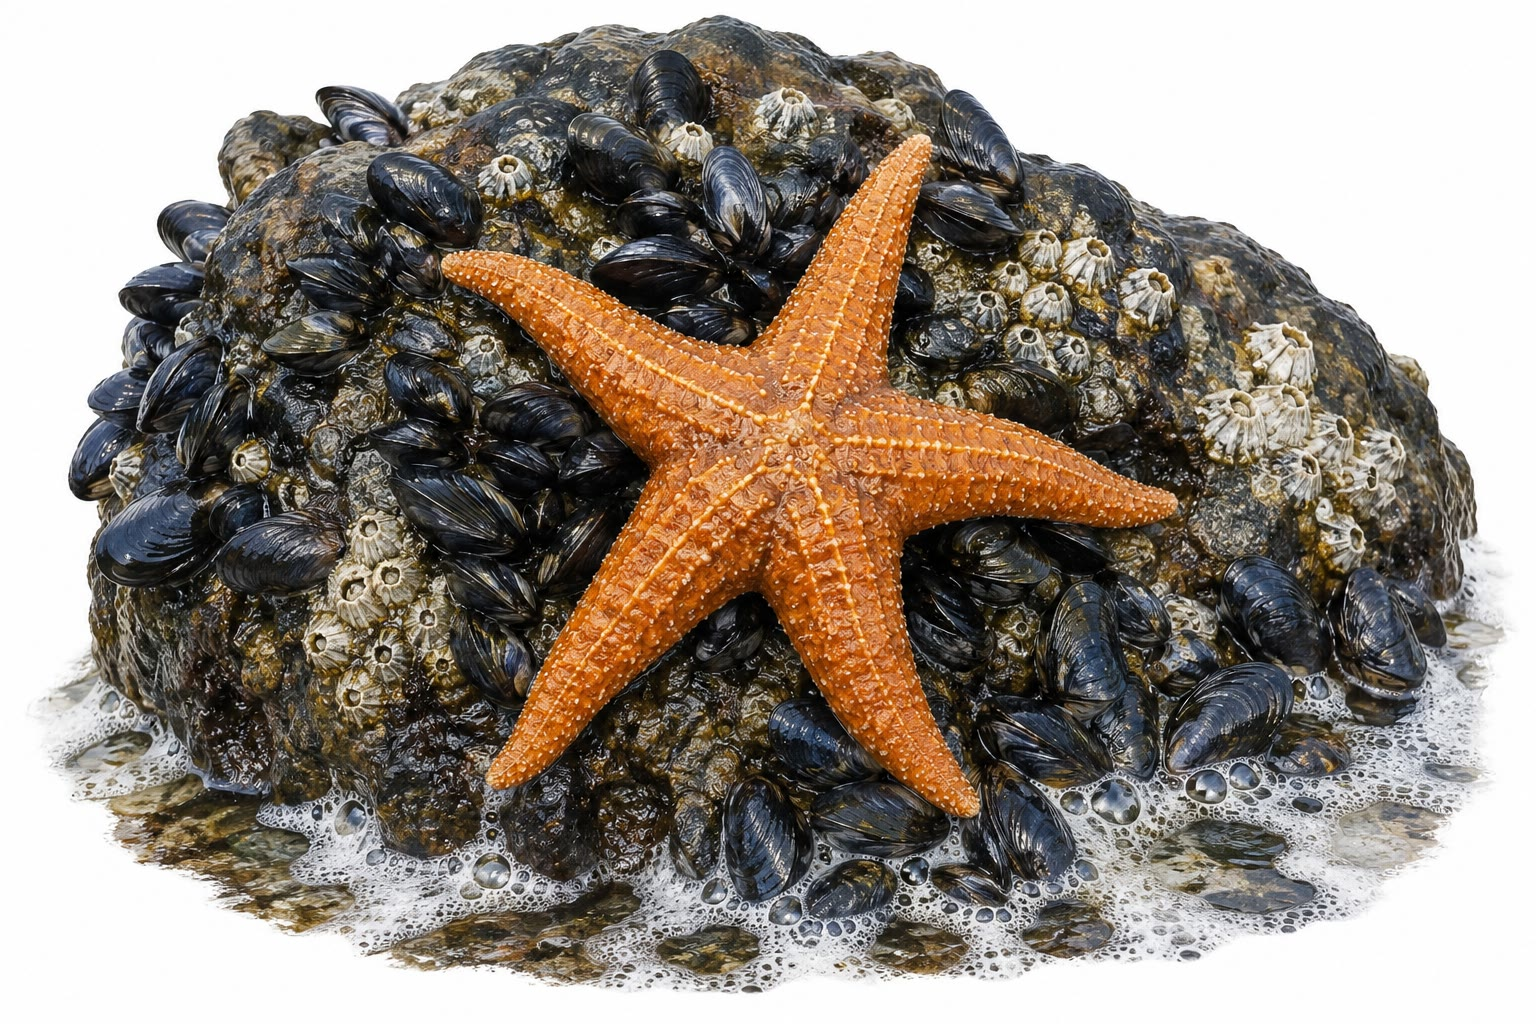
\includegraphics[width=0.6\linewidth]{images/book3/ai/b3-27-sea-star-mussels.jpg}

{\small Une étoile de mer prédatrice sur un banc de moules à marée
basse~: le prédateur clé de voûte dont le retrait a transformé un estran
de quinze espèces en une monoculture de moules.}
\end{omfigure}

\section{Vivre ensemble~: parasitisme, mutualisme, commensalisme}

\begin{definition}[Parasitisme, symbiose, mutualisme]\label{def:b1:species-interactions:symbiosis}
\index{symbiose}\index{parasite}\index{lichen}
Un \emph{parasite} vit aux dépens d'un hôte, sur lui (ectoparasite~:
tique, pou, gui) ou en lui (endoparasite~: ténia, plasmodium du
paludisme, champignon de la rouille), en lui prenant des nutriments et
en réduisant sa valeur sélective sans nécessairement le tuer~; les
parasites sont souvent spécialisés, avec des cycles de vie complexes
passant par plusieurs hôtes. Une \emph{symbiose} est toute association
étroite et durable entre deux espèces~; un \emph{\omterm{def:b1:species-interactions:types}{mutualisme}} est une
symbiose profitable aux deux~: la \omterm{def:b1:plant-water-minerals:mycorrhiza}{mycorhize} (un champignon sur ou dans
les \omterm{def:b1:flowering-plant-organization:organs}{racines} d'une plante, qui échange phosphate et eau contre du sucre~;
\cref{ch:b1:plant-water-minerals}), la \omterm{def:b1:plant-water-minerals:nodules}{nodosité} racinaire (des
bactéries fixatrices d'azote nourries par la légumineuse), le
\emph{lichen} (un champignon hébergeant une algue ou une
cyanobactérie), le corail de récif (un cnidaire hébergeant des
dinoflagellés photosynthétiques), le microbiote intestinal d'un
ruminant ou d'un termite (\cref{ch:b1:digestion-absorption}), et la
pollinisation (du nectar contre un transport de pollen). Bien des
\omterm{def:b1:species-interactions:types}{mutualismes} ont commencé comme \omterm{def:b1:species-interactions:types}{parasitismes} ou \omterm{def:b1:species-interactions:types}{prédations} que la
coévolution des partenaires a tournés au bénéfice mutuel, et ils
restent conditionnels~: un champignon mycorhizien dans un sol riche en
phosphate est un coût, et la plante le réduit.
\end{definition}

\begin{example}[La pollinisation comme échange]\label{ex:b1:species-interactions:pollination}
Une fleur dépense quelques joules de sucre en nectar~; une abeille
dépense du vol pour le récolter et porte du pollen de fleur en fleur
chemin faisant. La couleur, le parfum, la forme et le calendrier de la
fleur s'adressent à ses pollinisateurs, et la longueur de langue de
l'abeille, sa vision des couleurs et sa mémoire de butinage s'adressent
à ses fleurs~; certains couples sont si étroitement ajustés --- un long
éperon nectarifère et l'unique papillon dont la trompe l'atteint ---
qu'aucun des deux ne survit sans l'autre, et toute une communauté
végétale peut dépendre de quelques espèces d'insectes.
\end{example}

\begin{omfigure}
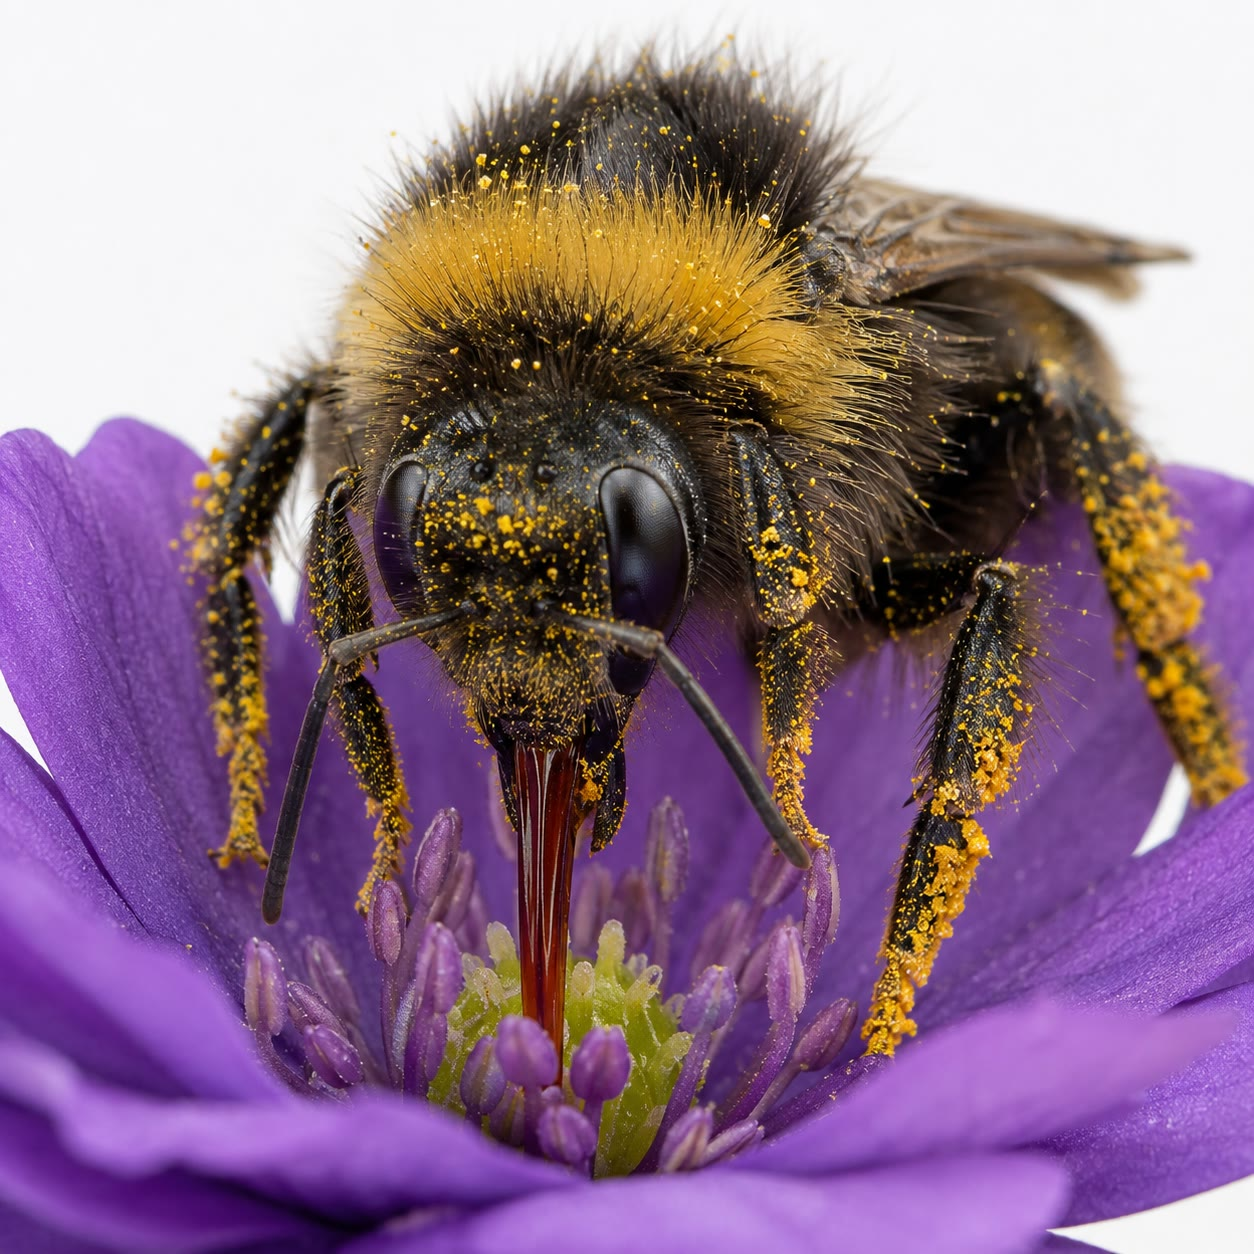
\includegraphics[width=0.56\linewidth]{images/book3/ai/b3-27-bee-flower.jpg}

{\small Un \omterm{def:b1:species-interactions:types}{mutualisme} à l'œuvre~: du nectar pour l'abeille, un transport
de pollen pour la fleur. La forme de chaque partenaire a été façonnée
par l'autre.}
\end{omfigure}

\begin{remark}[Le commensalisme est rare et instable]\label{rem:b1:species-interactions:commensal}
Peu d'interactions sont vraiment $+/0$~: l'épiphyte qui ombrage son
hôte, le rémora qui coûte à son requin un peu de traînée, le héron
garde-bœufs qui mange ce que le bétail dérange ne sont commensaux qu'à
la précision de la mesure près. Les interactions se classent par leur
effet net, et l'effet net peut changer avec les conditions.
\end{remark}

\section{Les interactions qui façonnent la biocénose}

\begin{definition}[Espèce clé de voûte, cascade trophique]\label{def:b1:species-interactions:keystone}
\index{espece cle de voute@espèce clé de voûte}\index{cascade trophique}
Une \emph{espèce clé de voûte} est une espèce dont l'effet sur la
\omterm{def:b1:ecosystem-organization:ecosystem}{biocénose} est sans commune mesure avec son abondance ou sa biomasse~:
retirez-la et la structure de la \omterm{def:b1:ecosystem-organization:ecosystem}{biocénose} change, d'ordinaire parce
qu'elle contrôlait une compétitrice dominante. Une \emph{cascade
trophique} est la propagation d'un effet le long d'une \omterm{def:b1:ecosystem-organization:foodweb}{chaîne
alimentaire} sur plus d'un niveau~: la présence d'un prédateur abaisse
les herbivores, ce qui élève les plantes~; son retrait fait l'inverse.
Les cascades montrent que les \omterm{def:b1:ecosystem-organization:ecosystem}{biocénoses} sont structurées par le haut
autant que par le bas (par la productivité,
\cref{ch:b1:ecosystem-organization}).
\end{definition}

\begin{proposition}[Un prédateur peut entretenir la diversité]\label{prop:b1:species-interactions:paine}
En mangeant l'espèce qui gagnerait autrement la \omterm{def:b1:species-interactions:types}{compétition} pour
l'espace ou les ressources, un prédateur maintient les perdantes dans
la \omterm{def:b1:ecosystem-organization:ecosystem}{biocénose}~; son retrait laisse la compétitrice dominante les exclure,
et la diversité chute.
\end{proposition}
\begin{proof}[Faits expérimentaux]
Paine (1966) retira l'étoile de mer \emph{Pisaster} d'une portion de
\qty{8}{m} de côte rocheuse du Pacifique nord-américain et laissa une
portion voisine comme témoin. L'étoile de mer mange moules, balanes et
autres animaux fixés, les moules de préférence. En deux ans, la moule
\emph{Mytilus} s'était étendue vers le bas du rocher et en avait pris
presque tout l'espace~; les balanes, chitons, patelles et algues qui
vivaient dans les intervalles disparurent, et les quinze espèces de la
parcelle témoin tombèrent à huit. La part du prédateur dans la biomasse
de la \omterm{def:b1:ecosystem-organization:ecosystem}{biocénose} était faible~; son retrait changea tout.
\end{proof}

\begin{omfigure}
\begin{tikzpicture}
\begin{axis}[
  width=0.74\linewidth, height=5.6cm,
  axis x line=bottom, axis y line=left,
  xmin=1963, xmax=1969, ymin=0, ymax=18,
  xlabel={année}, ylabel={espèces sur la parcelle},
  xlabel style={font=\small}, ylabel style={font=\small},
  tick label style={font=\small}, xtick={1963,1964,1965,1966,1967,1968},
  x tick label style={/pgf/number format/1000 sep=},
  legend style={font=\scriptsize, at={(0.98,0.03)}, anchor=south east, draw=none, fill=none},
  legend cell align=left,
]
\addplot[omDef, very thick, mark=*] coordinates {(1963,15) (1964,15) (1965,14) (1966,15) (1967,15) (1968,15)};
\addlegendentry{témoin~: étoile de mer présente}
\addplot[omThm, very thick, mark=square*] coordinates {(1963,15) (1964,12) (1965,10) (1966,9) (1967,8) (1968,8)};
\addlegendentry{étoile de mer retirée}
\node[font=\scriptsize, anchor=south west, align=left] at (axis cs:1966.2,10.6) {les moules prennent\\ le rocher};
\end{axis}
\end{tikzpicture}

{\small L'expérience de retrait de Paine (d'après ses données). La
diversité de la parcelle privée de prédateur tombe de moitié en cinq
ans tandis que le témoin garde ses quinze espèces.}
\end{omfigure}

\begin{example}[Loups, wapitis et saules]\label{ex:b1:species-interactions:wolves}
Les loups furent exterminés d'un grand parc de montagne dans les années
1920~; ses wapitis se multiplièrent et broutèrent jusqu'au moignon les
saules et les trembles des berges~; les castors, qui ont besoin de
saule, se raréfièrent~; les passereaux perdirent leurs fourrés. Quand
les loups furent réintroduits en 1995, les wapitis déclinèrent et,
surtout, évitèrent les fonds de vallée où ils étaient vulnérables~; les
saules repoussèrent, les castors revinrent et bâtirent des barrages, et
les zones humides qu'ils créèrent ramenèrent poissons, amphibiens et
oiseaux. La cascade courut d'un carnivore à un herbivore puis aux
plantes, et de là à une douzaine d'espèces qui ne rencontrèrent jamais
un loup --- le temps qu'il fait, la chasse et d'autres prédateurs y
ayant contribué, la part des loups dans le changement se discute encore.
\end{example}

\begin{omfigure}
\begin{tikzpicture}[font=\footnotesize, >=Stealth, line cap=round,
  lv/.style={draw, thick, rounded corners=3pt, inner sep=4pt, align=center, fill=white, minimum width=2.6cm}]
  \node[lv, fill=omDef!25] (wolf) at (0,4.5) {loups};
  \node[lv, fill=omProp!20] (elk) at (0,2.8) {wapitis};
  \node[lv, fill=omExo!20] (willow) at (0,1.1) {saules, trembles};
  \node[lv, fill=omProp!20] (beaver) at (3.8,1.1) {castors};
  \node[lv, fill=omDef!12] (wet) at (7.4,1.1) {mares, zones humides};
  \node[lv, fill=omThm!15] (birds) at (3.8,-0.6) {passereaux, poissons,\\ amphibiens};
  \draw[->, very thick, omThm] (wolf) -- (elk) node[midway, right] {$-$~: moins nombreux, et tenus loin des berges};
  \draw[->, very thick, omThm] (elk) -- (willow) node[midway, left] {$-$~: broutage};
  \draw[->, very thick, omDef] (willow) -- (beaver) node[midway, above=9pt] {$+$~: nourriture, barrages};
  \draw[->, very thick, omDef] (beaver) -- (wet) node[midway, above] {$+$};
  \draw[->, very thick, omDef] (willow) -- (birds) node[midway, below left] {$+$};
  \draw[->, very thick, omDef] (wet) |- (birds) node[pos=0.8, below] {$+$};
  \node[anchor=north, align=center, gray] at (3.4,-1.5) {deux signes moins font un plus~: le retour des loups a fait croître les saules,\\ et les saules ont porté l'effet à des espèces que les loups n'ont jamais touchées};
\end{tikzpicture}

{\small Une \omterm{def:b1:species-interactions:keystone}{cascade trophique}~: un effet qui descend trois niveaux et
se propage latéralement dans la \omterm{def:b1:ecosystem-organization:ecosystem}{biocénose}. Les signes donnent le sens
de chaque lien.}
\end{omfigure}

\begin{omfigure}
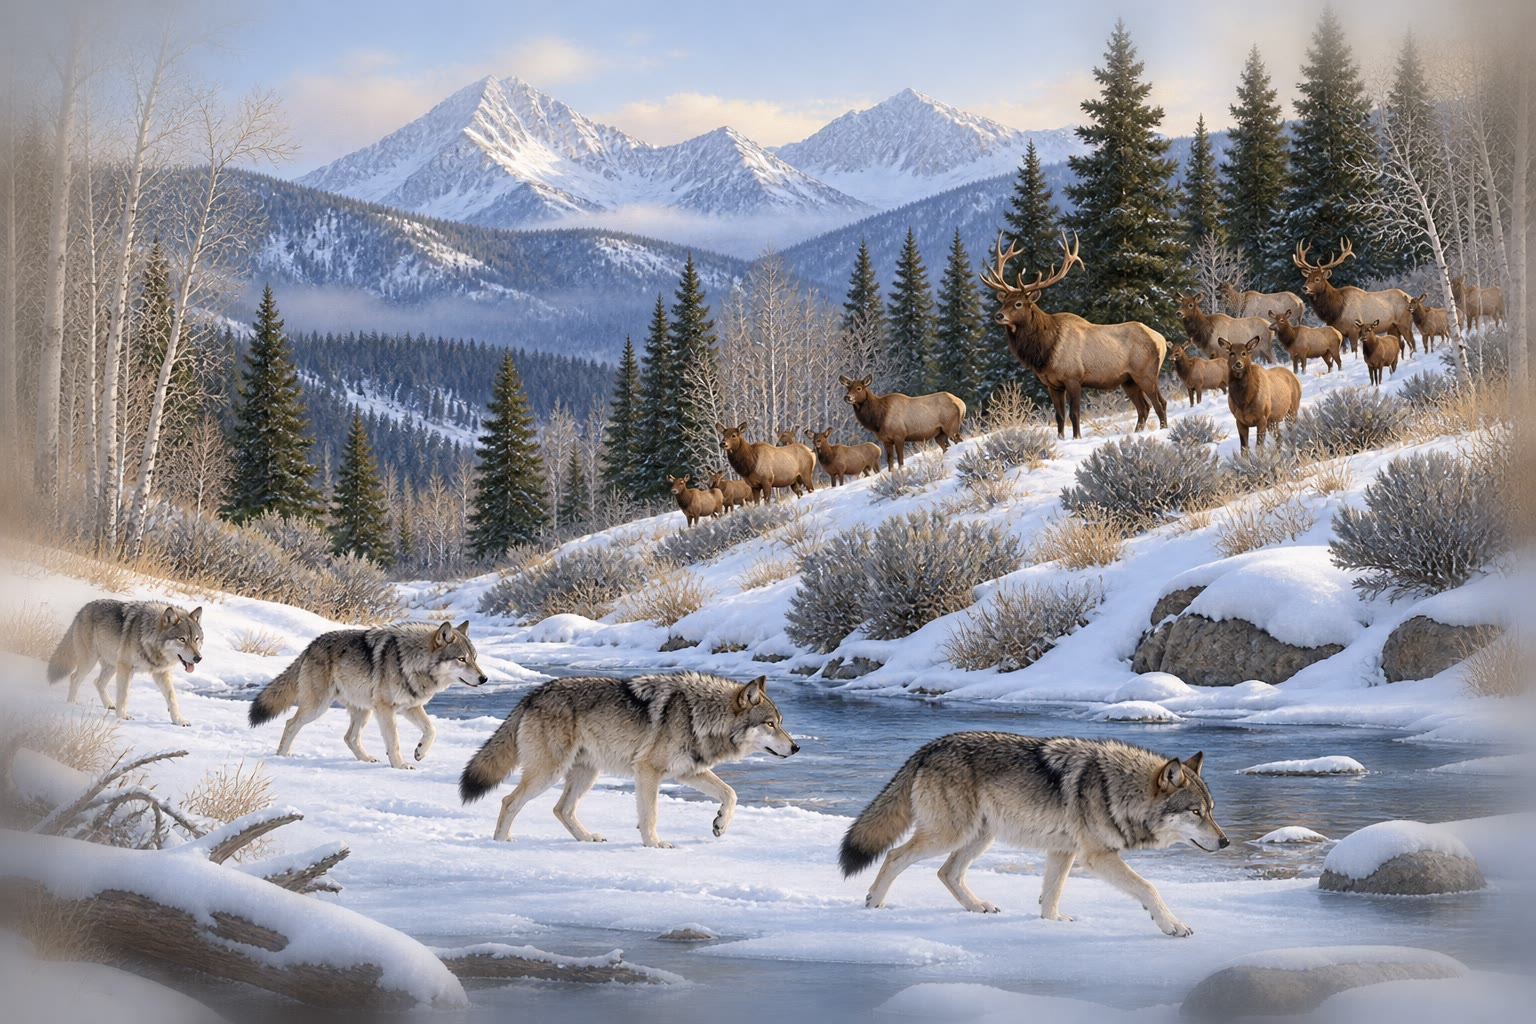
\includegraphics[width=0.6\linewidth]{images/book3/ai/b3-27-wolves-elk.jpg}

{\small Des loups et des wapitis dans une vallée en hiver. L'effet du
prédateur sur la végétation passe autant par les lieux où les wapitis
osent brouter que par leur nombre.}
\end{omfigure}

\begin{method}[Lire une interaction dans une expérience]\label{met:b1:species-interactions:reading}
\begin{enumerate}
  \item Repérer la manipulation (retrait, ajout, cage d'exclusion, mise
        en culture commune) et le témoin maintenu à côté dans les mêmes
        conditions.
  \item Pour chaque espèce, comparer son abondance avec et sans le
        partenaire~: le signe de la différence donne le signe de
        l'interaction sur cette espèce.
  \item Chercher les effets indirects~: une espèce qui a changé sans
        toucher à celle que l'on a manipulée est au bout d'une chaîne
        --- trouver les intermédiaires.
  \item Vérifier l'échelle de temps (une \omterm{def:b1:species-interactions:types}{compétition} peut demander bien
        des générations pour se résoudre~; une cascade court à la
        vitesse du niveau le plus lent) et l'échelle d'espace (le
        résultat tient-il au-delà de la parcelle~?).
  \item Ajuster le modèle quand les données le permettent~: courbes
        logistiques et \omterm{prop:b1:species-interactions:lotka}{isoclines} pour la \omterm{def:b1:species-interactions:types}{compétition}, \omterm{thm:b1:species-interactions:holling}{équation du disque}
        pour une \omterm{def:b1:species-interactions:functional}{réponse fonctionnelle}, et lire les paramètres sur les
        tracés linéarisés.
\end{enumerate}
\end{method}

\section{Exercices}

\begin{exercise}[$\star$]\label{exo:b1:species-interactions:1}
Donner le couple de signes et un exemple pour chacun des six types
d'interaction.
\end{exercise}

\begin{exercise}[$\star$]\label{exo:b1:species-interactions:2}
Énoncer le principe d'\omterm{def:b1:species-interactions:competition}{exclusion compétitive} et dire pourquoi il
n'interdit pas cinq fauvettes dans un même épicéa.
\end{exercise}

\begin{exercise}[$\star$]\label{exo:b1:species-interactions:3}
Définir le \omterm{def:b1:species-interactions:functional}{temps de manipulation} et le taux d'attaque, et donner le
taux d'ingestion maximal d'un prédateur pour $h = \qty{30}{min}$.
\end{exercise}

\begin{exercise}[$\star$]\label{exo:b1:species-interactions:4}
Qu'est-ce qu'une \omterm{def:b1:species-interactions:keystone}{espèce clé de voûte}~? Pourquoi n'est-ce pas simplement
la plus abondante~?
\end{exercise}

\begin{exercise}[$\star\star$]\label{exo:b1:species-interactions:5}
L'espèce 1 a $K_1 = 500$, l'espèce 2 a $K_2 = 400$, avec $\alpha =
0.5$ et $\beta = 0.6$. Tracer les \omterm{prop:b1:species-interactions:lotka}{isoclines} et donner l'issue.
Reprendre avec $\alpha = 2$, $\beta = 0.6$.
\end{exercise}

\begin{exercise}[$\star\star$]\label{exo:b1:species-interactions:6}
Un prédateur de $a = \qty{0.2}{m^2/h}$ et $h = \qty{0.25}{h}$ rencontre
des proies à \qty{10}{} et \qty{100}{} par mètre carré. Calculer son
taux d'ingestion dans chaque cas et la densité à laquelle il est à
demi-saturation.
\end{exercise}

\begin{exercise}[$\star\star$]\label{exo:b1:species-interactions:7}
Pourquoi une réponse de type III stabilise-t-elle une \omterm{def:b1:populations:population}{population} de
proies à basse densité alors qu'une réponse de type II ne le fait pas~?
\end{exercise}

\begin{exercise}[$\star\star$]\label{exo:b1:species-interactions:8}
À partir de l'expérience de Gause, expliquer pourquoi \emph{P.~bursaria}
a coexisté avec \emph{P.~aurelia} mais non \emph{P.~caudatum}. Qu'est-ce
qui a fait la différence~: le taux de croissance ou la \omterm{def:b1:ecosystem-organization:niche}{niche}~?
\end{exercise}

\begin{exercise}[$\star\star$]\label{exo:b1:species-interactions:9}
Un mime batésien devient plus commun que son modèle toxique. Prévoir ce
qu'il advient de la protection des deux, et pourquoi le succès du mime
se limite lui-même.
\end{exercise}

\begin{exercise}[$\star\star\star$]\label{exo:b1:species-interactions:10}
La parcelle de retrait de Paine a perdu sept espèces. Expliquer, à
l'aide du modèle des \omterm{prop:b1:species-interactions:lotka}{isoclines}, comment un prédateur qui mange la
compétitrice dominante convertit une exclusion en coexistence.
\end{exercise}

\begin{exercise}[$\star\star\star$]\label{exo:b1:species-interactions:11}
Un champignon mycorhizien prélève \qty{15}{\%} des photosynthétats
d'une plante et lui fournit \qty{80}{\%} de son phosphate. Dans quelles
conditions l'association est-elle un \omterm{def:b1:species-interactions:types}{mutualisme}, et dans quelles
conditions un \omterm{def:b1:species-interactions:types}{parasitisme}~? Proposer une expérience pour trancher.
\end{exercise}

\begin{exercise}[$\star\star\star$]\label{exo:b1:species-interactions:12}
Concevoir une expérience pour éprouver si ce sont les loups, plutôt que
le temps qu'il fait ou la chasse, qui ont causé le rétablissement des
saules~: témoins, réplicats, variables à mesurer, et quel résultat
réfuterait la cascade.
\end{exercise}

\section{Problème~: le prédateur et l'estran}

\begin{problem}[{Problème du week-end --- les ciliés de Gause dans un
tube, les données d'ingestion d'un prédateur ajustées à l'équation du
disque, l'estran de Paine avec et sans son étoile de mer, et le bilan
d'un pollinisateur, jusqu'au taux d'attaque et au temps de manipulation
du prédateur}]
\label{pb:b1:species-interactions:1}

\medskip
\noindent\textbf{Partie I --- La \omterm{def:b1:species-interactions:types}{compétition} dans un tube.}
On cultive deux ciliés séparément~: l'espèce A atteint $K_A = 200$ par
\qty{0.5}{mL} avec $r_A = \qty{0.8}{d^{-1}}$~; l'espèce B atteint
$K_B = 130$ avec $r_B = \qty{0.55}{d^{-1}}$. Ensemble, un individu
de B consomme autant de nourriture que $\alpha = 1.4$ individus de A, et
un individu de A autant que $\beta = 0.9$ de B.
\begin{enumerate}
  \item Écrire les deux \omterm{prop:b1:species-interactions:lotka}{isoclines} et leurs intersections avec les axes.
  \item Les tracer et dire quelle espèce gagne, et pourquoi l'issue ne
        dépend pas des effectifs de départ.
  \item D'après les temps de doublement ($\ln 2/r$), quelle espèce
        aurait-on attendue gagnante d'après le seul taux de croissance~?
  \item Une troisième espèce C se nourrit au fond du tube et ne
        concurrence A que faiblement ($\alpha = 0.3$, $\beta = 0.3$, $K_C = 100$).
        Tracer les \omterm{prop:b1:species-interactions:lotka}{isoclines} et donner l'issue.
  \item Pourquoi le principe d'exclusion tient-il dans un tube et
        échoue-t-il si souvent dans une forêt~? Donner deux raisons.
  \item Calculer les effectifs d'équilibre de A et de C au croisement
        des \omterm{prop:b1:species-interactions:lotka}{isoclines}.
\end{enumerate}

\medskip
\noindent\textbf{Partie II --- L'\omterm{thm:b1:species-interactions:holling}{équation du disque}.}
On propose à un coléoptère prédateur des proies aux densités de 5, 10,
20, 40 et 80 par mètre carré~; il en mange respectivement 2,0, 3,3,
5,0, 6,7 et 8,0 par jour.
\begin{enumerate}[resume]
  \item Porter le taux d'ingestion en fonction de la densité et
        identifier le type de réponse.
  \item Calculer $1/f$ et $1/N$ pour chaque point et les porter en
        graphique.
  \item De la pente et de l'ordonnée à l'origine, tirer $a$ et $h$.
  \item Calculer le taux d'ingestion maximal et la densité de
        demi-saturation.
  \item À laquelle des cinq densités le coléoptère passe-t-il plus de
        la moitié de son temps à manipuler~?
  \item Les proies du coléoptère croissent logistiquement avec $r = \qty{0.1}{d^{-1}}$
        et $K = 200$. À quelle densité la croissance des proies (par
        mètre carré sans coléoptère) égale-t-elle la consommation du
        coléoptère s'il y en a un par mètre carré~? Cet équilibre
        est-il stable face à une légère hausse des proies~?
  \item Une seconde espèce de proie apparaît, que le coléoptère
        manipule deux fois plus vite. Prévoir le changement de son
        ingestion totale à haute densité.
\end{enumerate}

\medskip
\noindent\textbf{Partie III --- L'estran.}
Sur la parcelle témoin de Paine, la \omterm{def:b1:ecosystem-organization:ecosystem}{biocénose} comptait 15 espèces~; sur
la parcelle de retrait, le compte tomba à 15, 12, 10, 9, 8, 8 en cinq
ans, et le recouvrement du rocher par les moules passa de \qty{20}{\%}
à \qty{85}{\%}.
\begin{enumerate}[resume]
  \item Calculer l'\omterm{def:b1:ecosystem-organization:diversity}{indice de Shannon} d'une parcelle de 15 espèces
        également abondantes, et d'une parcelle de 8 espèces où les
        moules font \qty{85}{\%} des individus et où les sept autres se
        partagent le reste également.
  \item De quel facteur la diversité a-t-elle chuté~?
  \item Expliquer, avec les signes des interactions, pourquoi retirer
        une interaction $+/-$ (la \omterm{def:b1:species-interactions:types}{prédation} sur les moules) a renforcé
        une interaction $-/-$ (la \omterm{def:b1:species-interactions:types}{compétition} pour le rocher).
  \item L'étoile de mer faisait moins de \qty{1}{\%} de la biomasse de
        la parcelle. Pourquoi la biomasse est-elle un mauvais guide de
        l'importance d'une espèce~?
  \item Prévoir ce qui serait arrivé si la proie préférée de l'étoile
        de mer avait été l'espèce la plus rare et non la dominante.
  \item Proposer un moyen de confirmer que c'était bien la \omterm{def:b1:species-interactions:types}{prédation}
        sur les moules et non quelque autre effet de l'étoile de mer
        (une expérience de mise en cage).
\end{enumerate}

\medskip
\noindent\textbf{Partie IV --- Le bilan d'un \omterm{def:b1:species-interactions:types}{mutualisme}.}
Une abeille visite 1000 fleurs en une journée et récolte \qty{40}{mg}
de sucre~; chaque fleur donne \qty{40}{\micro g} de sucre en nectar et
reçoit du pollen de 3 fleurs précédentes en moyenne par visite. La
plante consacre \qty{1}{\%} de ses photosynthétats quotidiens
(\qty{4}{mg} de sucre par fleur) au nectar~; le vol d'une abeille coûte
\qty{0.5}{mg} de sucre par heure de butinage (\qty{8}{h}).
\begin{enumerate}[resume]
  \item Calculer le gain net quotidien de sucre de l'abeille et son
        équivalent énergétique à \qty{16}{kJ/g}.
  \item Calculer le coût quotidien de la plante par fleur en fraction
        de ses photosynthétats et dire ce qu'il lui achète.
  \item Pourquoi cette interaction est-elle $+/+$ alors même que chaque
        partenaire exploite l'autre~?
  \item Un voleur de nectar mord la base de la fleur et prend le nectar
        sans toucher le pollen. Donner les signes de l'interaction
        voleur--plante et son effet probable sur l'abeille.
  \item Tracer le diagramme des signes entre la plante, l'abeille, le
        voleur et un oiseau qui mange les voleurs, et prédire l'effet
        indirect de l'oiseau sur la plante.
  \item Énoncer le résultat~: le taux d'attaque et le \omterm{def:b1:species-interactions:functional}{temps de
        manipulation} du coléoptère, et son taux d'ingestion maximal.
\end{enumerate}
\end{problem}
